\documentclass[a4paper, 12pt]{report}

\usepackage[italian]{babel}
\usepackage{graphicx}
\usepackage{float}
\usepackage{tabularx}
\usepackage{ltablex}
\usepackage[font=small,format=plain,labelfont=bf,up,textfont=normal,up,justification=justified,singlelinecheck=false,skip=0.01\linewidth]{caption}
\renewcommand{\familydefault}{\sfdefault}

\title{"Progetto di una base di dati per la gestione del ciclo di vita del difetto nella produzione dell'elettrodomestico"}
\author{Castellucci Matteo\\Matricola 0000825436\\Anno accademico 2018-2019}
\date{\today}

\begin{document}

\maketitle

\tableofcontents

\chapter{Introduzione}
In questo progetto si vuole realizzare una base di dati a supporto della gestione dei difetti nella realizzazione dell'elettrodomestico,
chiudendo la "catena dell'informazione" tra cliente ed azienda nella fase terminale del ciclo di vita del prodotto. Lo scopo è fornire
all'azienda tutte le informazioni necessarie sugli elettrodomestici una volta arrivati nelle mani del cliente finale, così da poter
ottenere informazioni sul campo per quanto riguarda gli obiettivi attesi e disattesi. In particolar modo, l'attenzione è posta sull'elemento
principe per quanto rigurda l'analisi del comportamento di un bene di consumo: il difetto, in tutti i suoi aspetti. Sarà permesso a tutti gli
attori in gioco, tecnici, telefonisti, analisti dei dati e progettisti, di poter avere una visione a tutto tondo del problema che riguarda
il prodotto: le tempistiche di manifestazione, di risoluzione, il tipo di guasto ed altro ancora. Questo permetterà all'azienda di poter
avere più controllo sullo sviluppo e la messa in produzione di futuri progetti avendo a disposizione più informazioni strategiche.

\chapter{Analisi}

\section{Intervista}
Si vuole realizzare una base di dati che permetta di gestire tutte le informazioni che riguardano un guasto di un elettrodomestico.
L'azienda riceve telefonate da un cliente che vengono smistate ad un adeguato centro assistenza dove ciascuna verrà raccolta da un operatore.
Ogni centro assistenza ha sede in una città e possiede una determinata area di competenza, per cui tutte le chiamate che verranno effettuate
all'interno di quest'ultima verranno redirette al centro assistenza associato. L'identificazione dei centri assistenza viene fatta mediante dei
codici che hanno però valenza solamente nazionale.\newline
L'operatore, di cui l'azienda conosce dati identificativi come nome, cognome, data e luogo di nascita, codice fiscale, luogo di residenza, nonchè lo 
stipendio che gli elargisce, così come per ogni suo dipendente, chiede al cliente di identificarsi. Vengono richiesti dall'operatore 
il nome, il cognome e il recapito a cui fare riferimento nel momento nel quale un solo tecnico si recherà in loco per riparare il suo elettrodomestico. 
Eventualmente, l'operatore chiede anche l'indirizzo \textit{email}, qualora il cliente lo possieda. Inoltre, viene registrato il numero di telefono 
chiamante a cui verrà fatto riferimento anche in futuro come specifico per quel dato cliente.\newline
In seguito, l'operatore chiede quale prodotto o quali prodotti del cliente hanno subito un guasto e saranno l'oggetto della corrente richiesta di 
assistenza. L'operatore per ogni elettrodomestico ne chiede la categoria, il modello, specificato con un codice, e si fa leggere "PNC" (\textit{Product 
Number Code}) e "SNC" (\textit{Serial Number Code}), codici che lo identificano univocamente trattenendo informazioni sulle caratteristiche tecniche e
la data di produzione. L'operatore richiede inoltre la data di acquisto dell'elettrodomestico e la data di installazione dello stesso e le registra qualora 
il cliente le abbia a disposizione o se ne ricordi. In assenza di data di acquisto sarà compito del tecnico, una volta recatosi a casa del cliente, 
recuperare almeno questa informazione e in caso la garanzia del prodotto sia scaduta o non sia trovata, far pagare il cliente. Il cliente potrebbe avere 
aderito opzionalmente ad un programma di estensione della garanzia, identificato da un codice, informazione che deve fornire, se non fase in chiamata, 
almeno al momento della visita. Da ultimo, l'operatore chiede al cliente di farsi descrivere il guasto o i guasti subiti e registra la data corrente come data di apertura 
della pratica, ponendo lo stato dell'intervento come aperto e concorda con il cliente la data di visita del tecnico a casa per la riparazione.\newline
Un difetto è univocamente determinato da due codici, il "\textit{Component Code}", che identifica quale parte di un elettrodomestico viene affetto, e
il codice di tipo, che indica qual è nello specifico il tipo di difetto che il componente può subire. Ad ogni difetto sono associati i ricambi che sono 
necessari per poterlo sistemare, che potrebbero anche essere più di uno o nessuno, identificati da un codice, e il costo di ciascuno di essi, 
sia in termini di costo del ricambio stesso, che del costo di manodopera per l'installazione.\newline
Un tecnico, che afferisce ad un centro assistenza come l'operatore, si preoccuperà, una volta raccolte le informazioni necessarie dalla chiamata,
di recarsi a casa del cliente e registrare a sua volta una descrizione personale del guasto o dei guasti del cliente, dopodichè possibilmente li riparerà
e si preoccuperà di chiudere la richiesta di assistenza pendente. Specificherà anche il tempo che ha impiegato nel risolvere il problema del cliente
espresso in quarti d'ora. Un tecnico può lavorare direttamente per l'azienda o è assunto tramite un'impresa terza per l'azienda stessa. \newline
Un progettista di elettrodomestici dovrà poi periodicamente recuperare le informazioni riguardanti i guasti che si sono verificati sui prodotti che
gli competono, indicati dalla o dalle categorie di prodotto a cui è assegnato, e stilare classifiche che possano aiutare l'azienda a migliorare la produzione.

\section{Analisi ed eliminazione delle ambiguità}

\begin{tabularx}{\linewidth}{X|X}
	\hline
	\textbf{Termine presente nel testo} & \textbf{Sinonimo utilizzato}\\
	\hline
	\hline
	Elettrodomestico & Prodotto\\
	\hline
	Pratica & Intervento\\
	\hline
	Telefonata & Intervento\\
	\hline
	Richiesta di assistenza & Intervento\\
	\hline
	Chiamata & Intervento\\
	\hline
	Riparazione & Intervento\\
	\hline
	\caption{Associazioni termine-sinonimo per formulare specifiche non ambigue}
\end{tabularx}

Il termine "elettrodomestico" verrà da qui in avanti sostituito dal termine "prodotto", in quanto dotato di una più adeguato carattere di astrattezza
e generalità, benchè il caso in esame sia studiato su di un'azienda che produce elettrodomestici. I termini come "chiamata", "richiesta di
assistenza", "intervento" e loro sinonimi vengono tutti raccolti sotto il termine "intervento" poichè di fatto descrivono le varie fasi dello
stesso, dalla richiesta iniziale del cliente, alla visita del tecnico dell'assistenza, fino alla riparazione del prodotto indicato. Si intende
che ogni intervento sarà raccolto in un'unica pratica e perciò anche quest'ultimo termine indica lo stesso concetto.

\section{Definizione delle specifiche ed estrapolazione dei concetti}
Si vuole realizzare una base di dati che permetta di gestire tutte le informazioni che riguardano un \textbf{guasto} di un \textbf{prodotto}.
Un prodotto è univocamente identificato da una combinazione di codici detti "PNC" (\textit{Product Number Code}) e "SNC" (\textit{Serial Number Code}) ed è caratterizzato
da una \textbf{categoria} e un \textbf{modello} sotto forma di codice. Un prodotto possiede inoltre una data di acquisto e una di installazione, insieme ad 
un'\textbf{estensione di garanzia} identificata da un codice, informazioni che però possono essere disponibili o meno, a seconda che il \textbf{cliente}
che lo possiede ne abbia tenuto traccia o meno.\newline
Al verificarsi di un guasto, il cliente si preoccupa di chiamare l'assistenza clienti dell'azienda produttrice per richiedere un
\textbf{intervento}. Ogni cliente verrà identificato dal suo numero di telefono e verranno registrati il suo nome, il suo cognome,
il recapito presso il quale dispacciare il \textbf{tecnico} per la riparazione del prodotto ed opzionalmente il suo indirizzo \textit{email},
solamente nel caso il cliente lo possedesse.\newline
Il cliente parlerà con un \textbf{operatore}, che chiederà al cliente tutte le informazioni relative al prodotto o ai prodotti
che hanno subito un guasto insieme alle descrizioni dei guasti stessi che vengono anch'esse registrate. Viene inoltre concordata una data di
visita del tecnico affinchè possa riparare il prodotto. Infine, vengono registrati la data della chiamata del cliente e viene
aggiornato lo stato dell'intervento come aperto. Quando il tecnico visiterà il cliente, uno solo per intervento, registrerà una sua descrizione
del guasto per ognuno di essi e dopo averli riparati segnerà lo stato dell'intervento come chiuso. Indicherà anche il tempo speso per farlo in quarti d'ora.\newline
Un guasto è associato ad uno specifico \textbf{difetto}, il quale è univocamente determinato da due codici: il "\textit{Component Code}"
che identifica il \textbf{componente} del prodotto coinvolto e un codice che identifica il tipo del difetto su quello specifico componente. Nella
riparazione di un difetto possono essere utilizzati uno o più \textbf{ricambi}, ognuno dei quali è identificato da un codice e vi è associato
sia un costo di acquisto per il ricambio stesso che di manodopera per l'installazione.\newline
L'azienda possiede per i suoi dipendenti informazioni come il codice fiscale, il nome, il cognome, la data e il luogo di nascita, luogo di
residenza e lo stipendio percepito. I dipendenti presi in considerazione sono gli operatori, i tecnici e i
\textbf{progettisti}. Gli operatori e i tecnici afferiscono ad uno specifico \textbf{centro assistenza} dell'azienda,
mentre i progettisti sono interessati ad analizzare i dati dei guasti di una o più categorie di prodotto stilando delle classifiche. Un tecnico
inoltre può essere dipendente interno dell'azienda oppure no.\newline
Un centro assistenza ha sede in una città e possiede una determinata area di competenza, nella quale tutte le telefonate che vengono fatte
per l'assistenza vengono inoltrate a quello specifico centro. Esso è identificato da un codice univoco, ma solo nella nazione in cui si trova.\newline

\begin{tabularx}{\linewidth}{>{\hsize=0.375\hsize}X|X|>{\hsize=0.475\hsize}X}
	\hline
	\textbf{Termine} & \textbf{Descrizione} & \textbf{Collegamenti}\\
	\hline
	\hline
	Prodotto & Un elettrodomestico di un determinato modello che l'azienda ha rilasciato sul mercato ed è stato comprato da un cliente, per poi subire un guasto &
	Cliente,\newline Modello,\newline Guasto\\
	\hline
	Modello & Una classe di prodotti accomunata da caratteristiche comuni & Prodotto\\
	\hline
	Cliente & Una persona che ha acquistato un prodotto presso l'azienda e ha richiesto un intervento per quello specifico prodotto & Prodotto,\newline 
	Intervento\\
	\hline
	Guasto & Un problema di varia natura che si è verificato in uno specifico prodotto, causato da un difetto nel prodotto stesso, per cui viene
	richiesto un intervento. Sarà analizzato da un progettista & Prodotto,\newline Difetto,\newline Intervento,\newline Progettista\\
	\hline
	Intervento & Una richiesta fatta da un cliente per risolvere uno o più guasti subiti, sarà registrato da un operatore e risolto da un tecnico
	& Guasto,\newline Operatore,\newline Tecnico\\
	\hline
	Difetto & Una classe di guasti accomunati dal componente in cui il guasto si verifica e la natura del difetto stesso, possono essere utilizzati
	dei ricambi per poterlo riparare & Guasto,\newline Componente,\newline Ricambio\\
	\hline
	Componente & Una parte di un prodotto che può subire un guasto per un suo difetto di produzione & Guasto,\newline Difetto\\
	\hline
	Ricambio & Un componente di un prodotto che può essere utilizzato nella riparazione di un difetto & Prodotto,\newline Difetto\\
	\hline
	Operatore & Un dipendente dell'azienda che si preoccupa di aprire richieste di intervento, appartiene ad un determinato centro assistenza
	& Intervento,\newline Centro Assistenza\\
	\hline
	Tecnico & Un dipendente dell'azienda che si preoccupa di attendere ad interventi di manutenzione e chiudere le richieste pendenti, appartiene
	ad un centro assistenza & Intervento,\newline Centro Assistenza\\
	\hline
	Progettista & Un dipendente dell'azienda che si preoccupa di analizzare i dati sui guasti accaduti, ma solamente su alcuni tipi
	di prodotto & Guasto, Prodotto\\
	\hline
	Centro Assistenza & Parte dell'azienda volta all'impiego di operatori e tecnici di assistenza & Operatore,\newline Tecnico\\
	\hline
	Categoria & Un'insieme di prodotti che rappresentano lo stesso tipo di elettrodomestico (ad esempio: "Forno", "Lavatrice", ecc.) & Prodotto\\
	\hline
	Estensione di garanzia & Particolare programma che può essere scelto per un prodotto per prolungare il periodo per il quale si trova in garanzia & Prodotto\\
	\hline
	\caption{Glossario dei termini}
\end{tabularx}

\chapter{Analisi concettuale}

\section{Schema scheletro}

\begin{figure}[H]
	\centering
	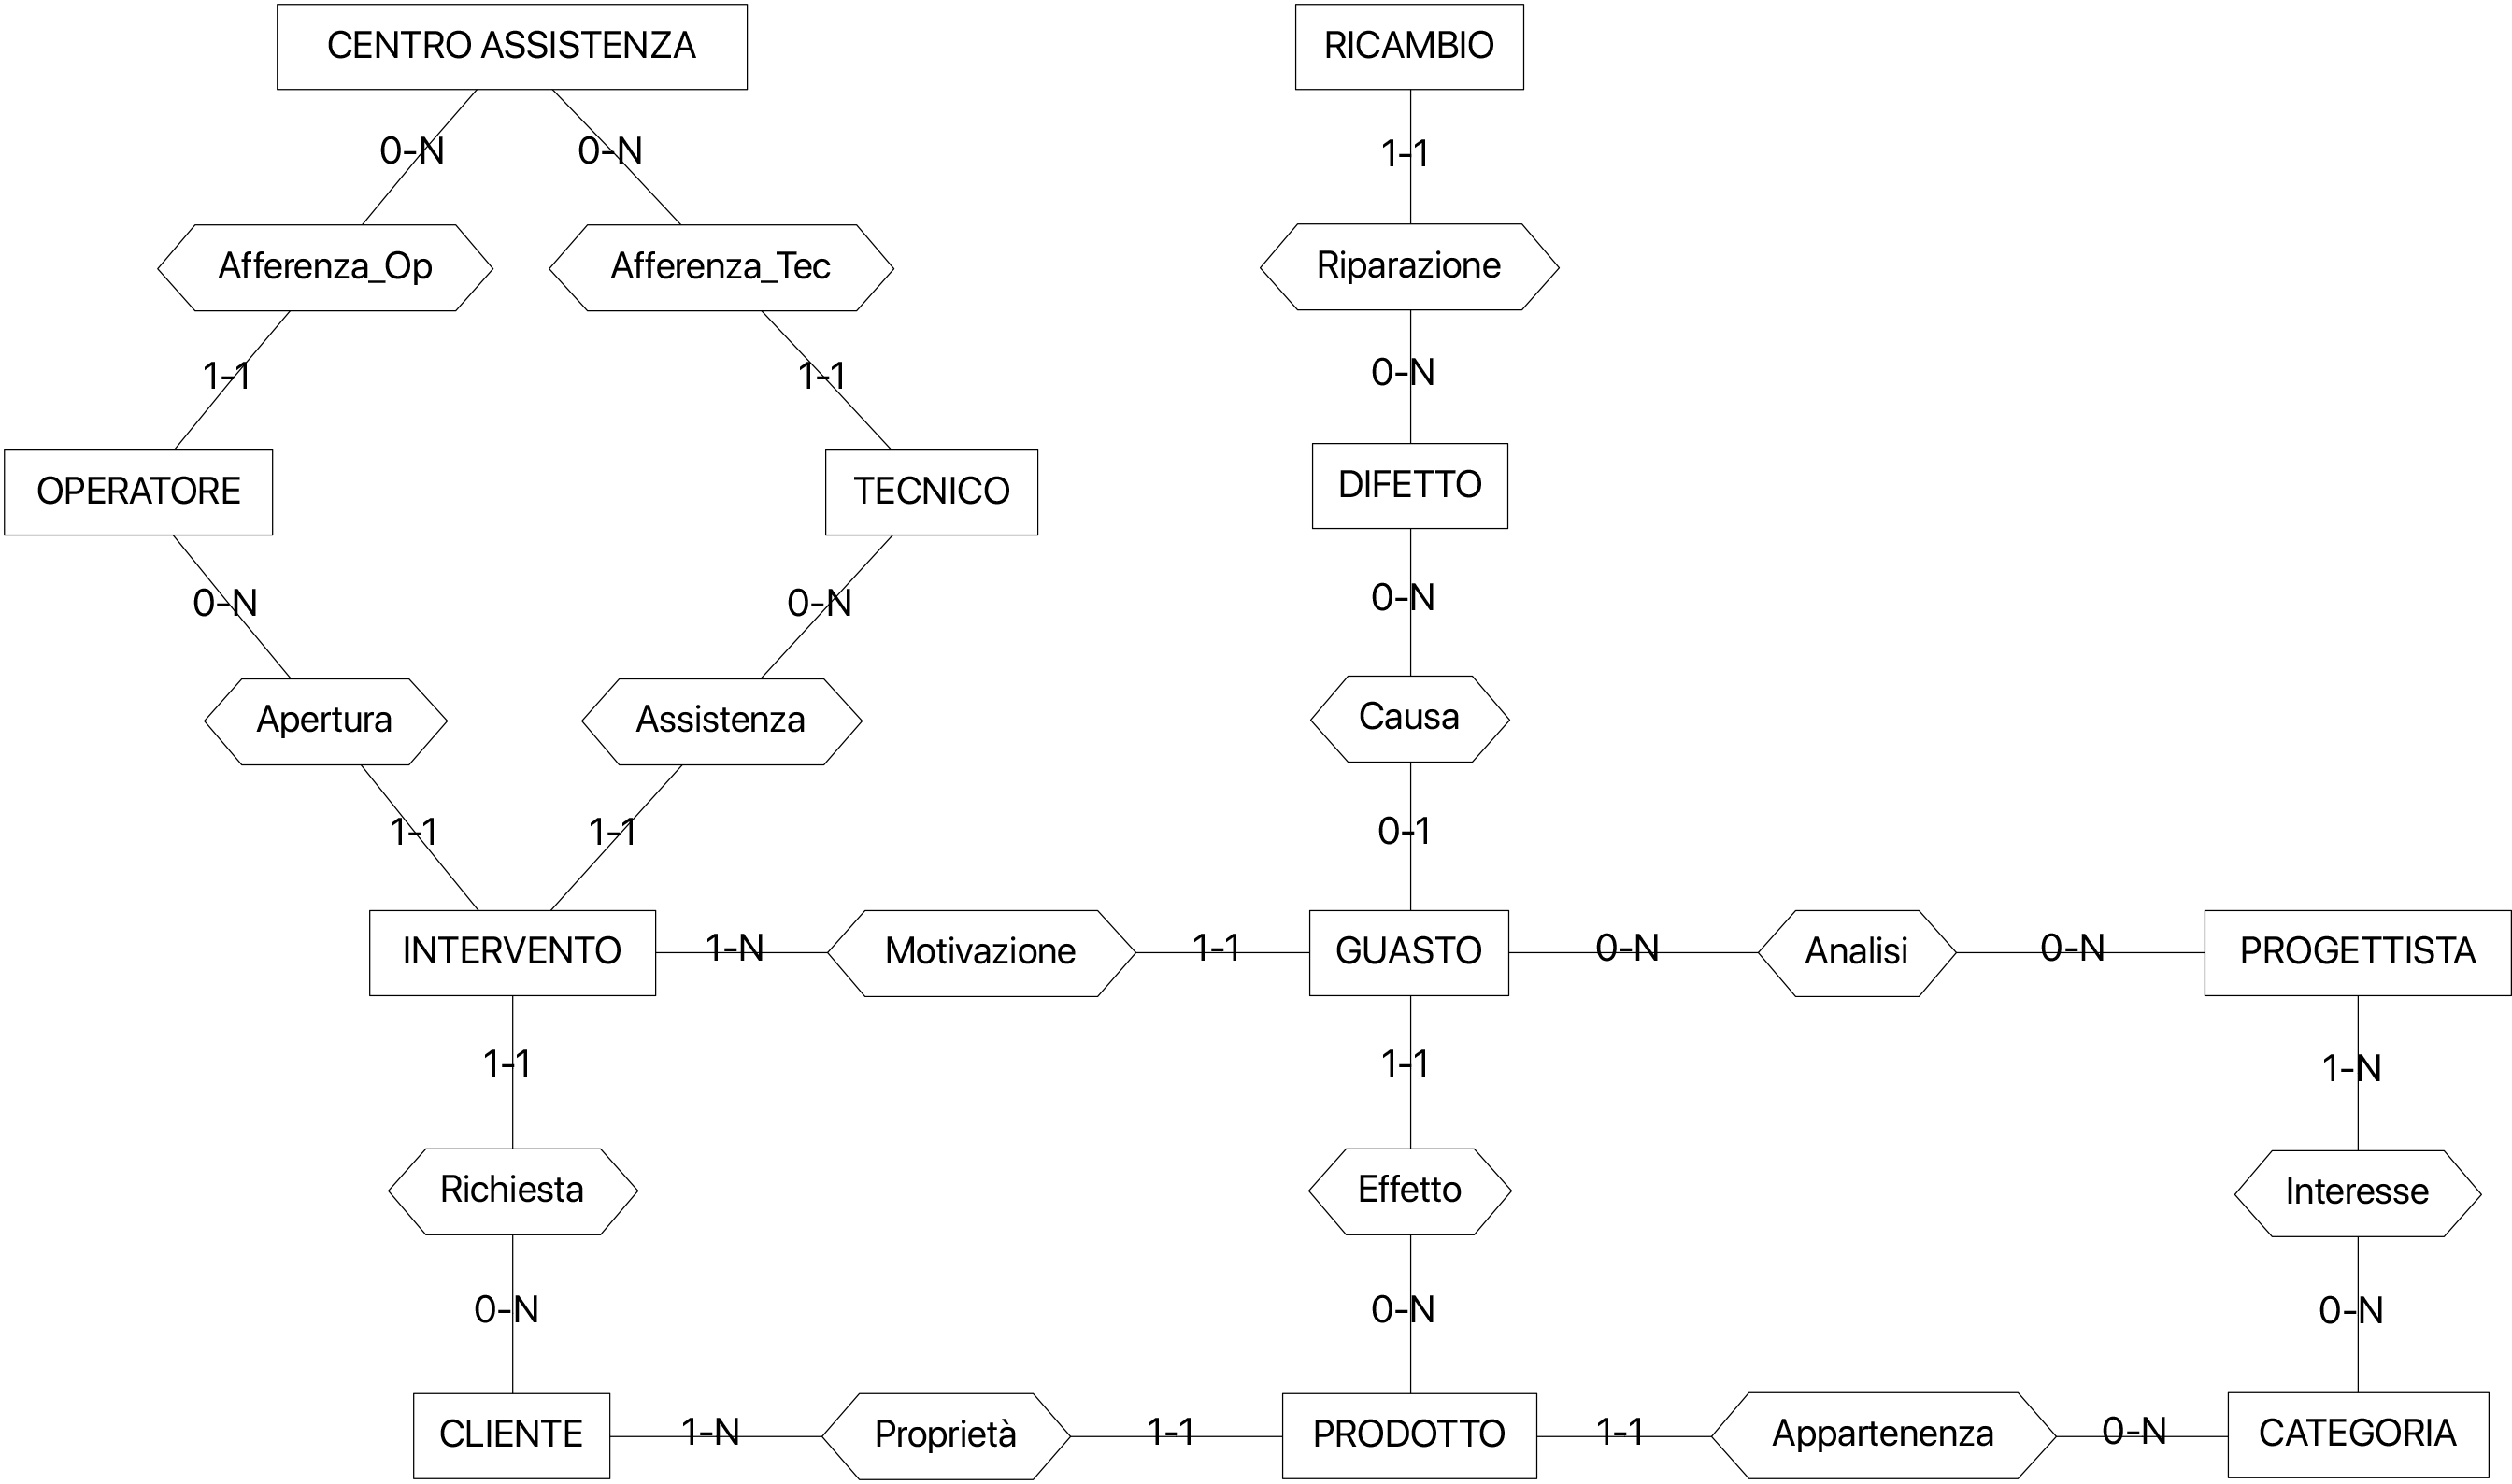
\includegraphics[width=\linewidth]{images/skeleton.png}
	\caption{Schema scheletro dei concetti più rilevanti estrapolati dalle specifiche}
\end{figure}

\section{Raffinamenti proposti}

\subsection{Gerarchia di persone}

Nelle specifiche sono specificati quattro concetti - "cliente", "operatore", "tecnico" e "progettista" - che si prestano a diventare entità, ma
che ruotano tutte attorno alla nozione di persona. Tutte queste infatti sono persone e in quanto tali condividono almeno informazioni come il nome
ed il cognome; è perciò significativo metterle assieme in una gerarchia che discende da persona. Inoltre, tutti e tre i concetti meno che "cliente"
sono di fatto dipendenti dell'azienda e in quanto tali le informazioni che l'azienda trattiene su di essi sono le stesse, pur intrattenendo con gli
altri concetti rapporti diversi a seconda della mansione che svolgono. Anche per queste tre concetti è opportuno raccoglierli attraverso una seconda
gerarchia che origini da dipendente, che a sua volta è una persona. I concetti di "operatore" e "tecnico" saranno poi legati a "centro assistenza"
così come individuato nello schema scheletro. Il "progettista", poichè può occuparsi o di una o di più categorie di prodotto quando analizza i "guasti",
queste gli verranno associate mediante un attributo multiplo obbligatorio. Pur essendo condivise tra più "progettisti" e anche dai "prodotti" stessi,
non è il caso separare il concetto di "categoria" in un'entità a sè stante, perchè non presenta nessuna caratteristica che non sia il suo nome stesso
e in caso l'insieme dei prodotti che presentano una stessa categoria dovesse essere rimosso, non è problematico. Infatti, significherebbe semplicemente
che l'azienda ha deciso di voler smettere di trattare le informazioni su una determinata categoria di elettrodomestici e a maggior ragione anche la
categoria stessa è bene che non lasci traccia nel \textit{database}.

\begin{figure}[H]
	\centering
	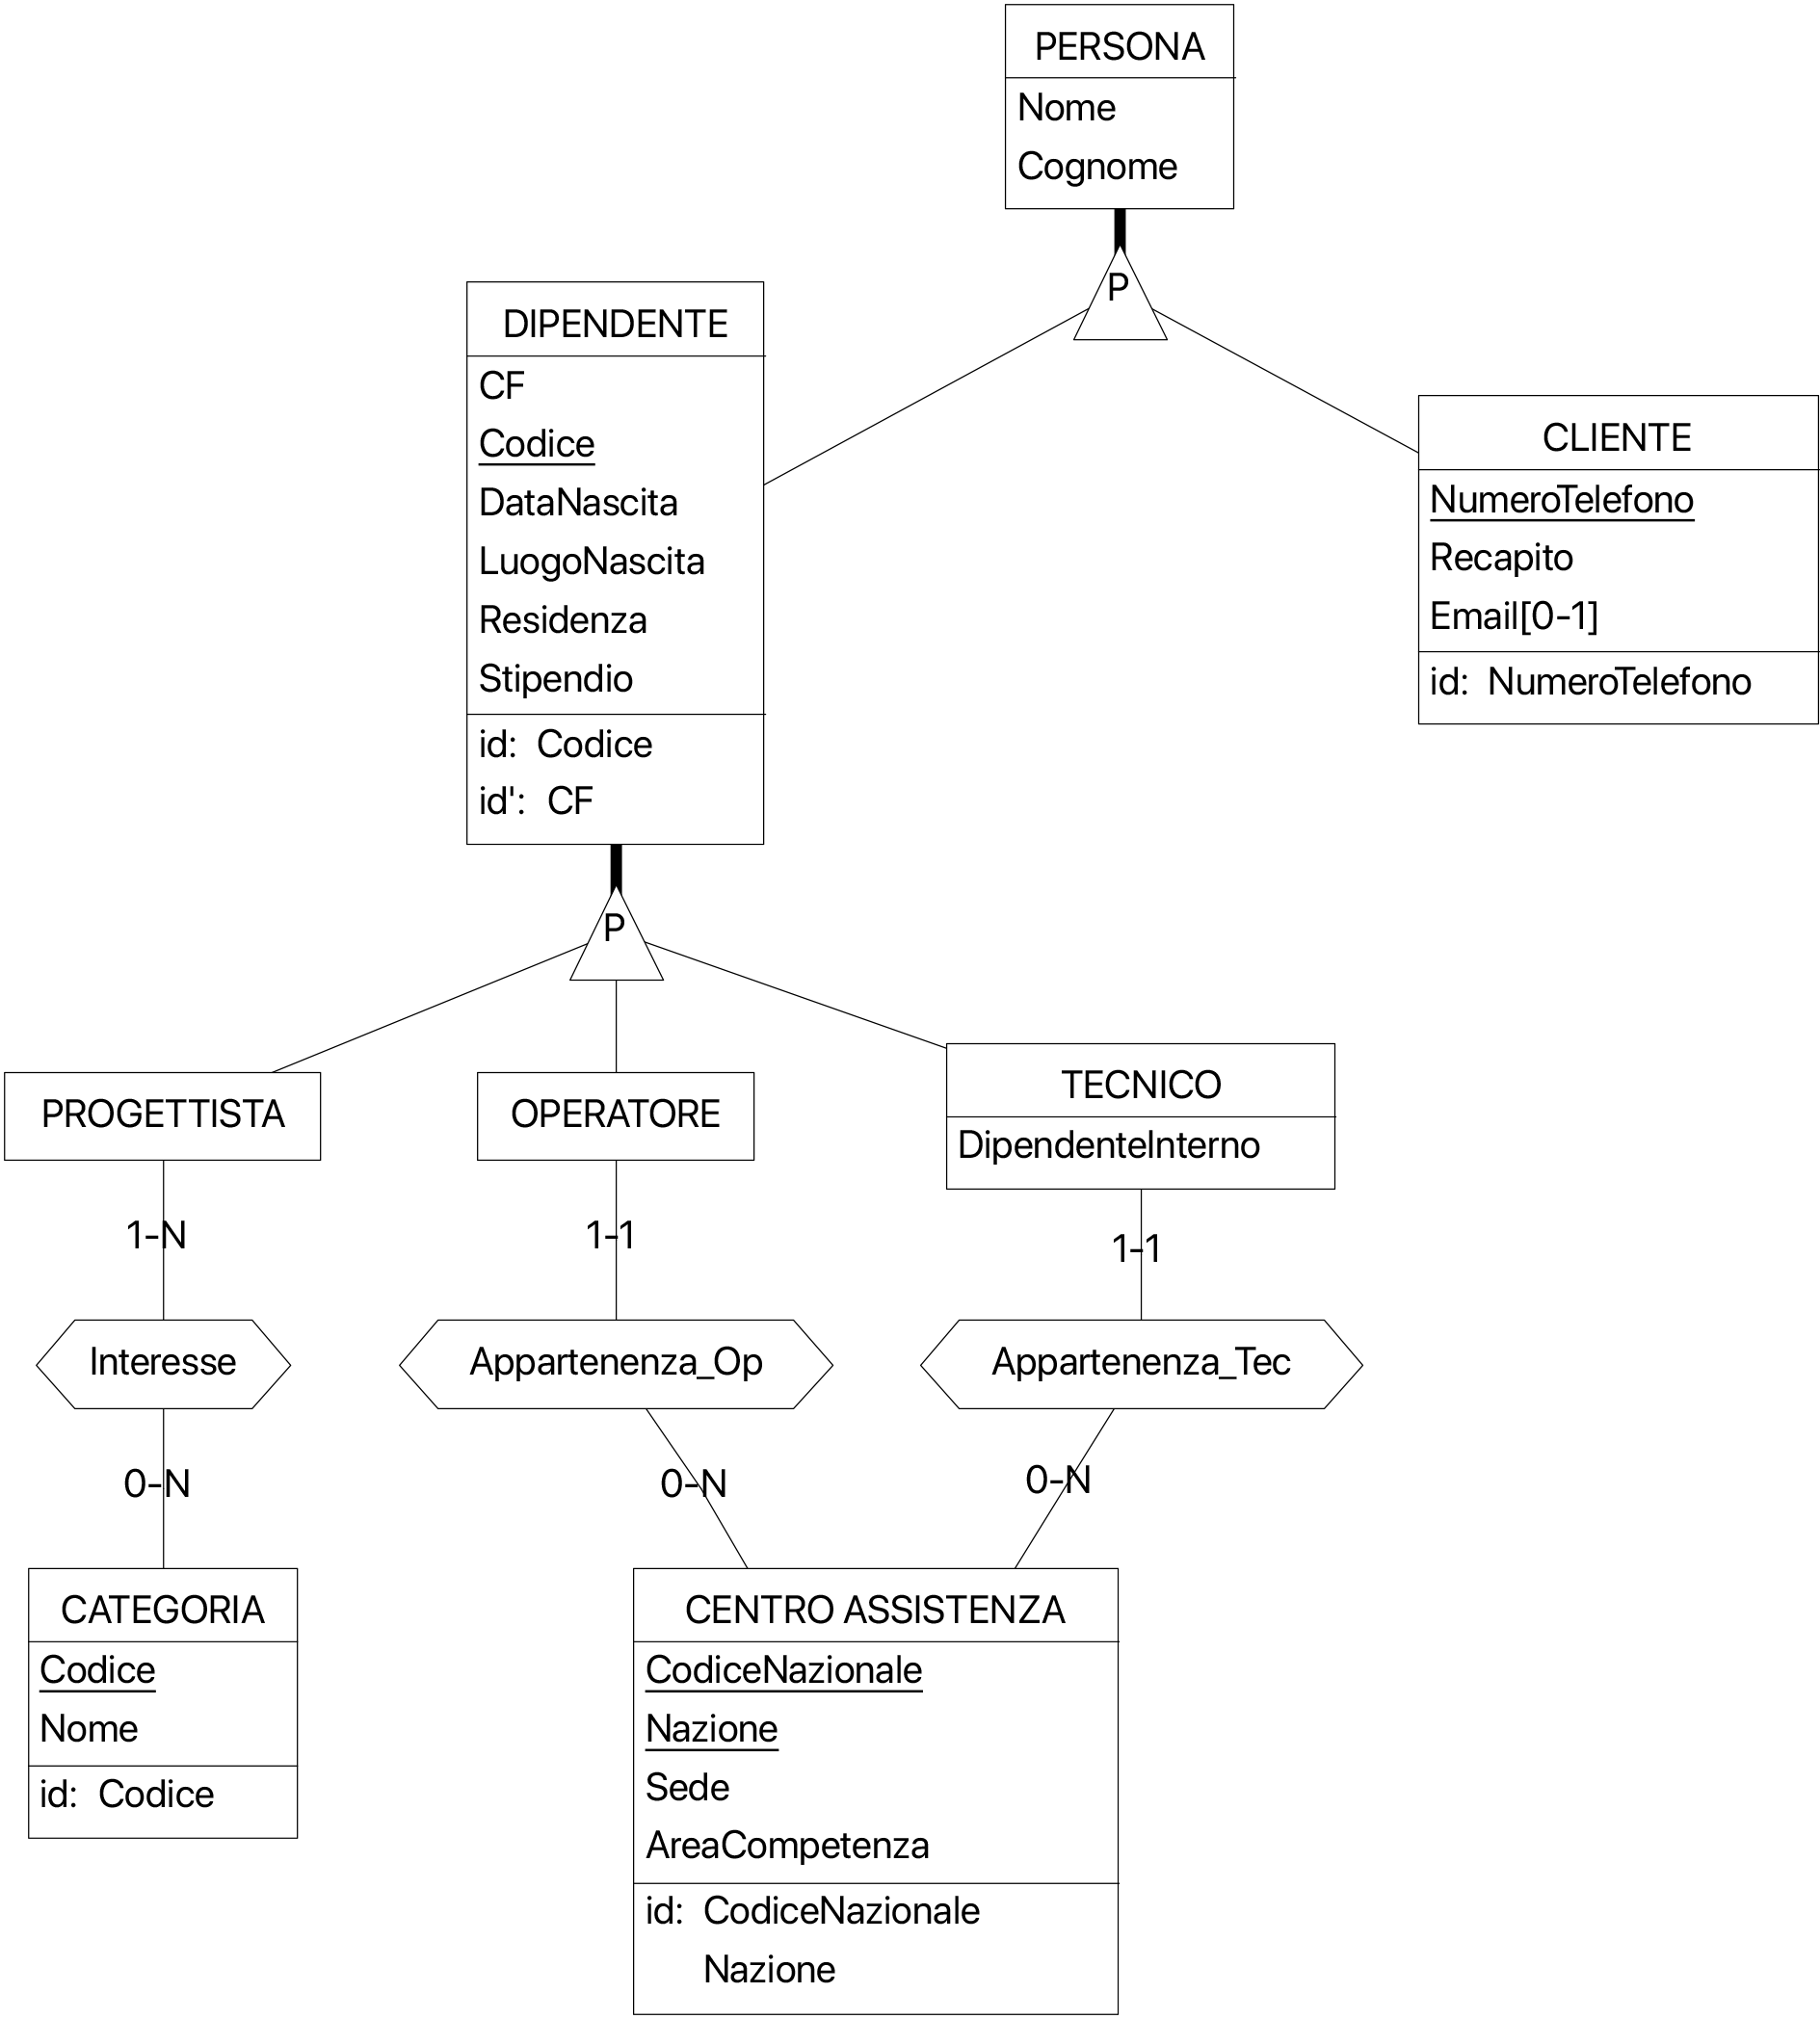
\includegraphics[width=\linewidth]{images/persone.png}
	\caption{Schema raffinato dei concetti riguardanti "persone"}
\end{figure}

\subsection{Necessità di un entità separata per i guasti}

Dai concetti di "persone" è poi immediato spostarsi sui quelli di "intervento" e "guasto" che li coinvolgono più direttamente. Benchè il testo
specifichi che siano i prodotti, a causa dei loro guasti, ad essere in numero di uno o più presenti in un intervento, è più adatto frapporre il
concetto di "guasto" tra essi e quello di "intervento". È infatti facile immaginare come un cliente potrebbe voler riportare la presenza
di un guasto solamente dopo che un secondo si è verificato, magari perchè il primo non era così urgente, e lo farebbe all'interno dello stesso intervento.
Se eliminassimo il concetto di "guasto" questo non sarebbe possibile e inoltre provocherebbe problemi anche con la nozione di "difetto". Essendo
un prodotto caratterizzato anche da più guasti, infatti, potrebbero essere più di uno i difetti legati ad un prodotto, anche ripetuti nel tempo,
ma una schematizzazione del genere impedirebbe proprio la loro ripetizione. Potrebbe ad esempio verificarsi un guasto diverso in un momento successivo,
che verrà incluso poi in un intervento successivo, ma la cui origine è sempre lo stesso difetto di progettazione.\newline I dati che sono di competenza del tecnico
inserire sono tutti modellati mediante attributi opzionali, poichè si suppone che l'apertura della pratica coincida con l'inserimento di un nuovo
\textit{record} nel \textit{database}, momento nel quale questi dati sono ancora sconosciuti. Per le nozioni di "componente" e "garanzia" è stato
deciso di non renderle entità poichè non possiedono caratteristiche interessanti che non siano i codici stessi che le identificano. Inoltre, un componente
è esso stesso un ricambio, solo acquistato in un secondo momento dalla costruzione dell'elettrodomestico.

\begin{figure}[H]
	\centering
	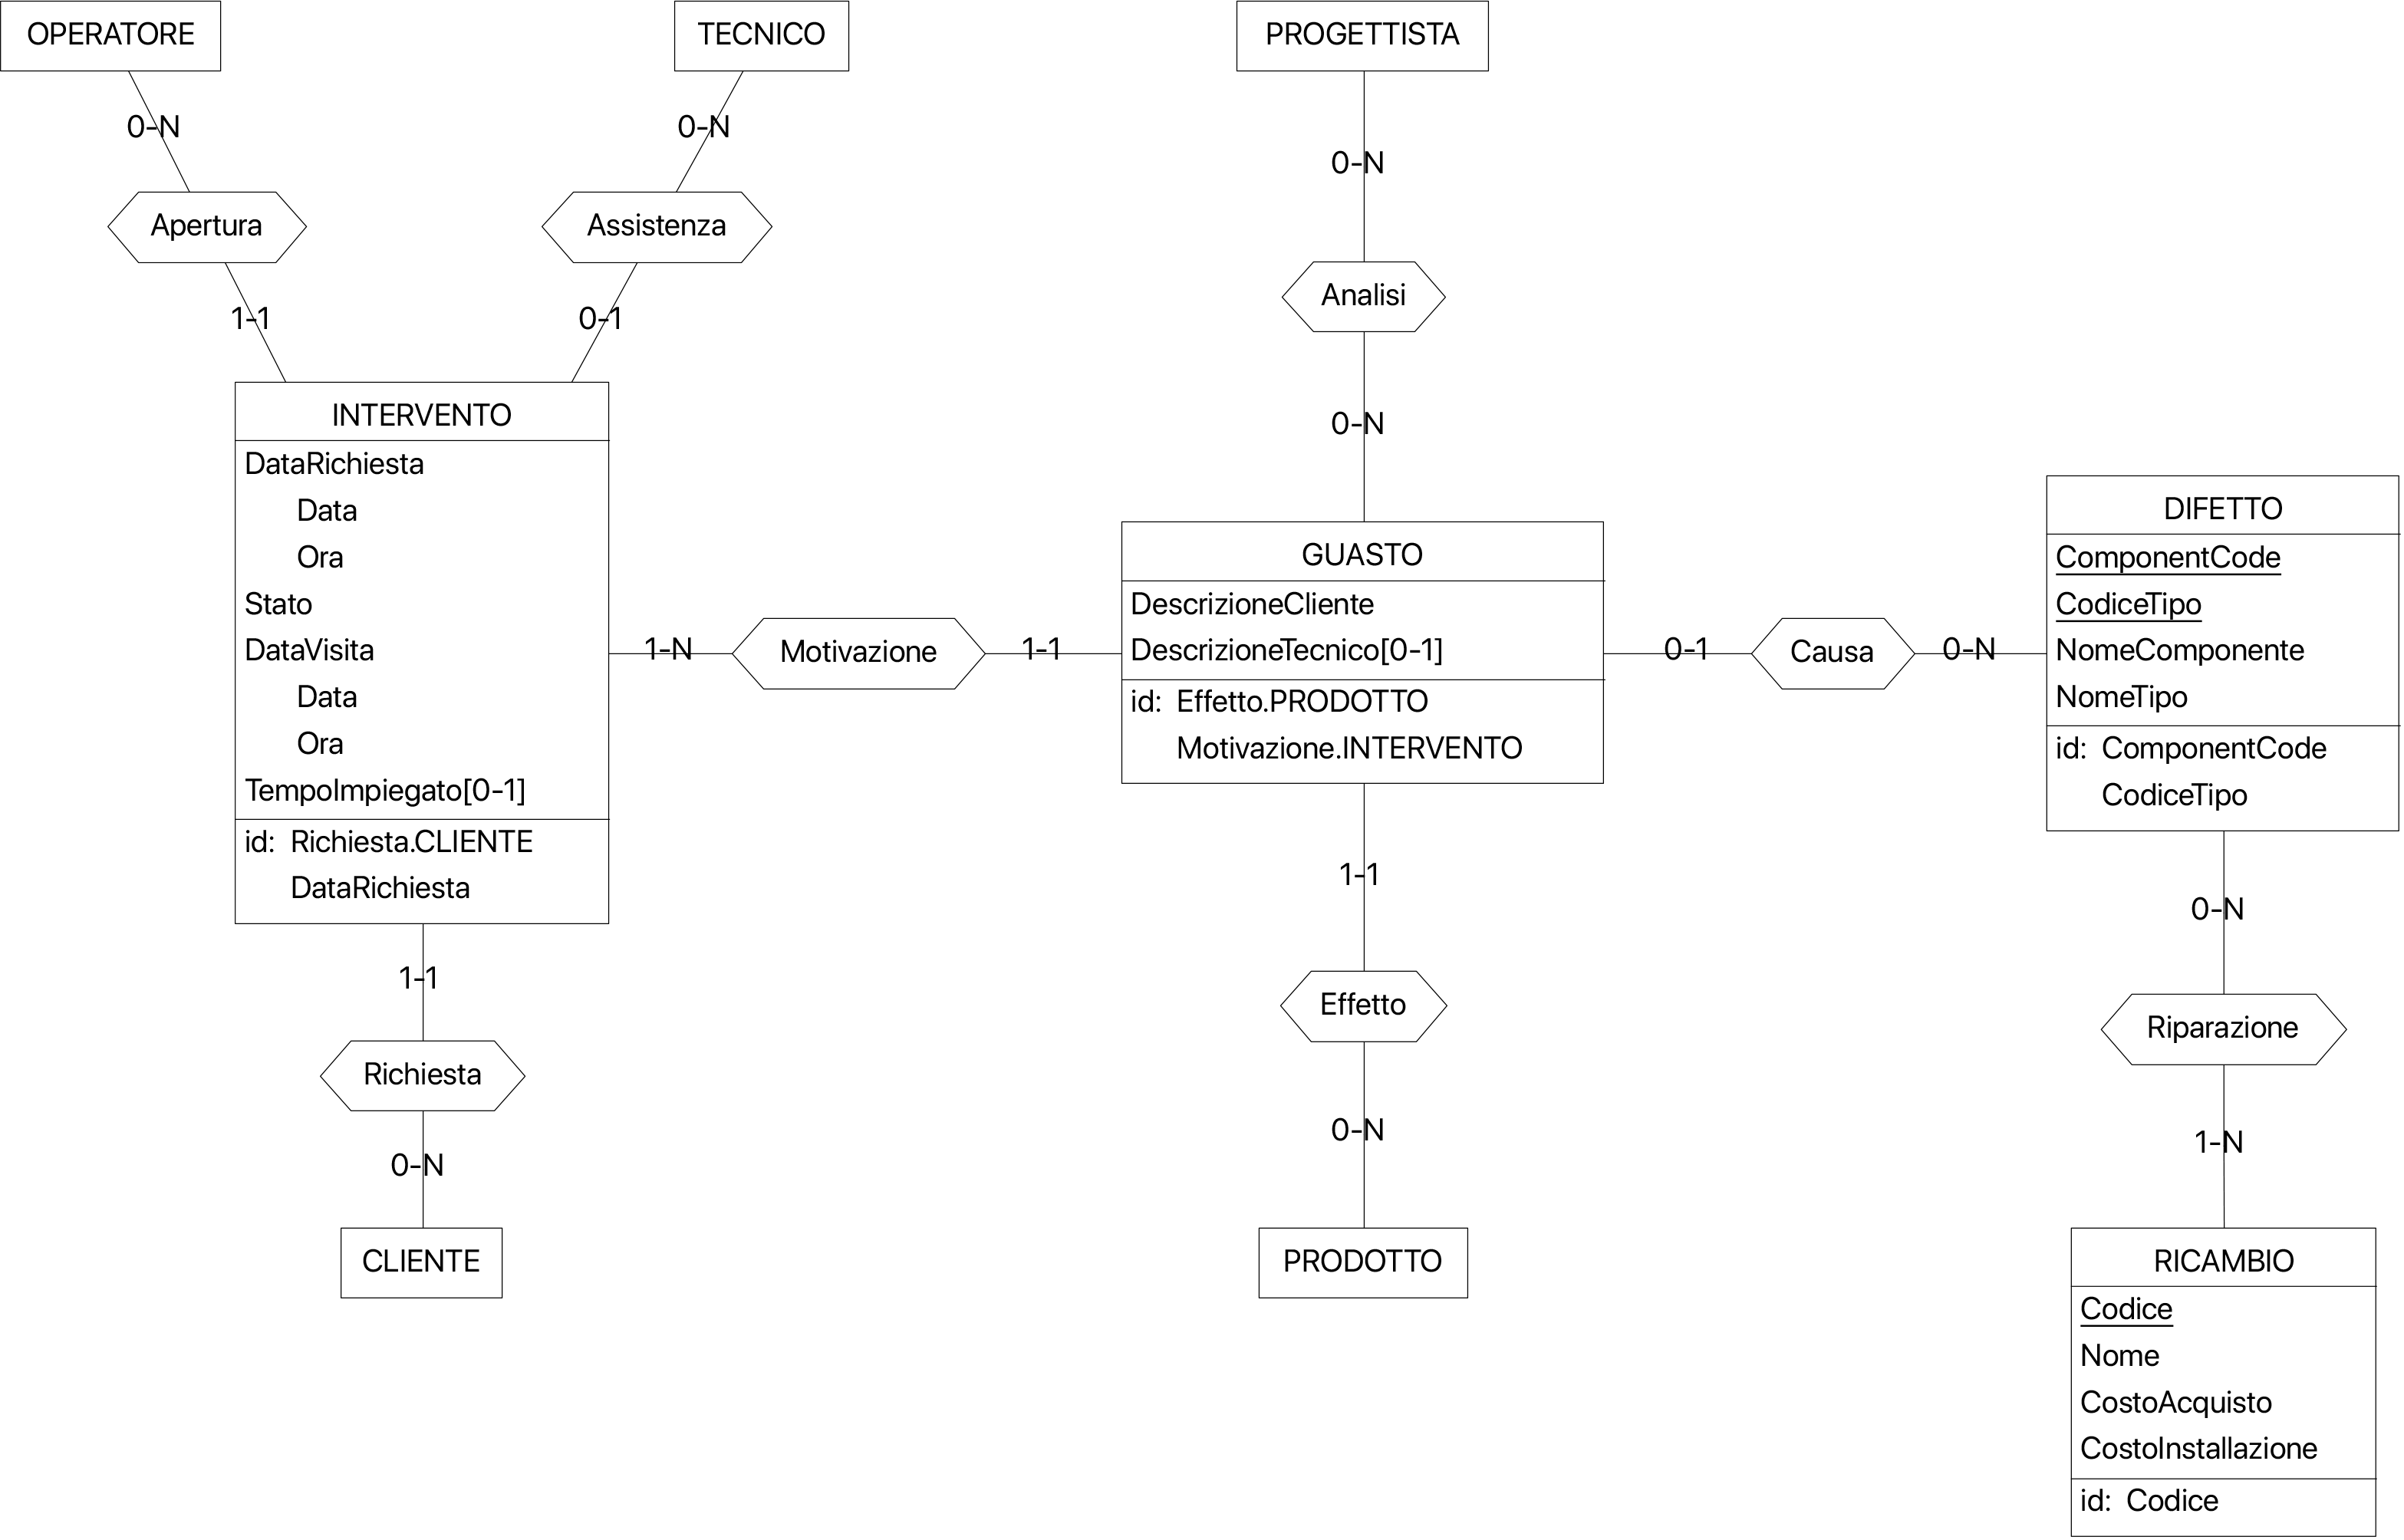
\includegraphics[width=\linewidth]{images/interventi.png}
	\caption{Schema raffinato dei concetti "intervento", "guasto" e "difetto"}
\end{figure}

\subsection{Modellazione del concetto di "prodotto"}

Da ultimo, espandiamo la nozione di "prodotto". Non è una componente dello schema particolarmente significativa, anche se presenta alcune particolarità.
Il fatto che il cliente possa non avere a disposizione le informazioni riguardanti la data di acquisto, installazione o addirittura la garanzia sul
prodotto, richiede una modellazione specifica. In particolar modo, queste informazioni sarà necessario modellarle come attributi singoli opzionali.

\begin{figure}[H]
	\centering
	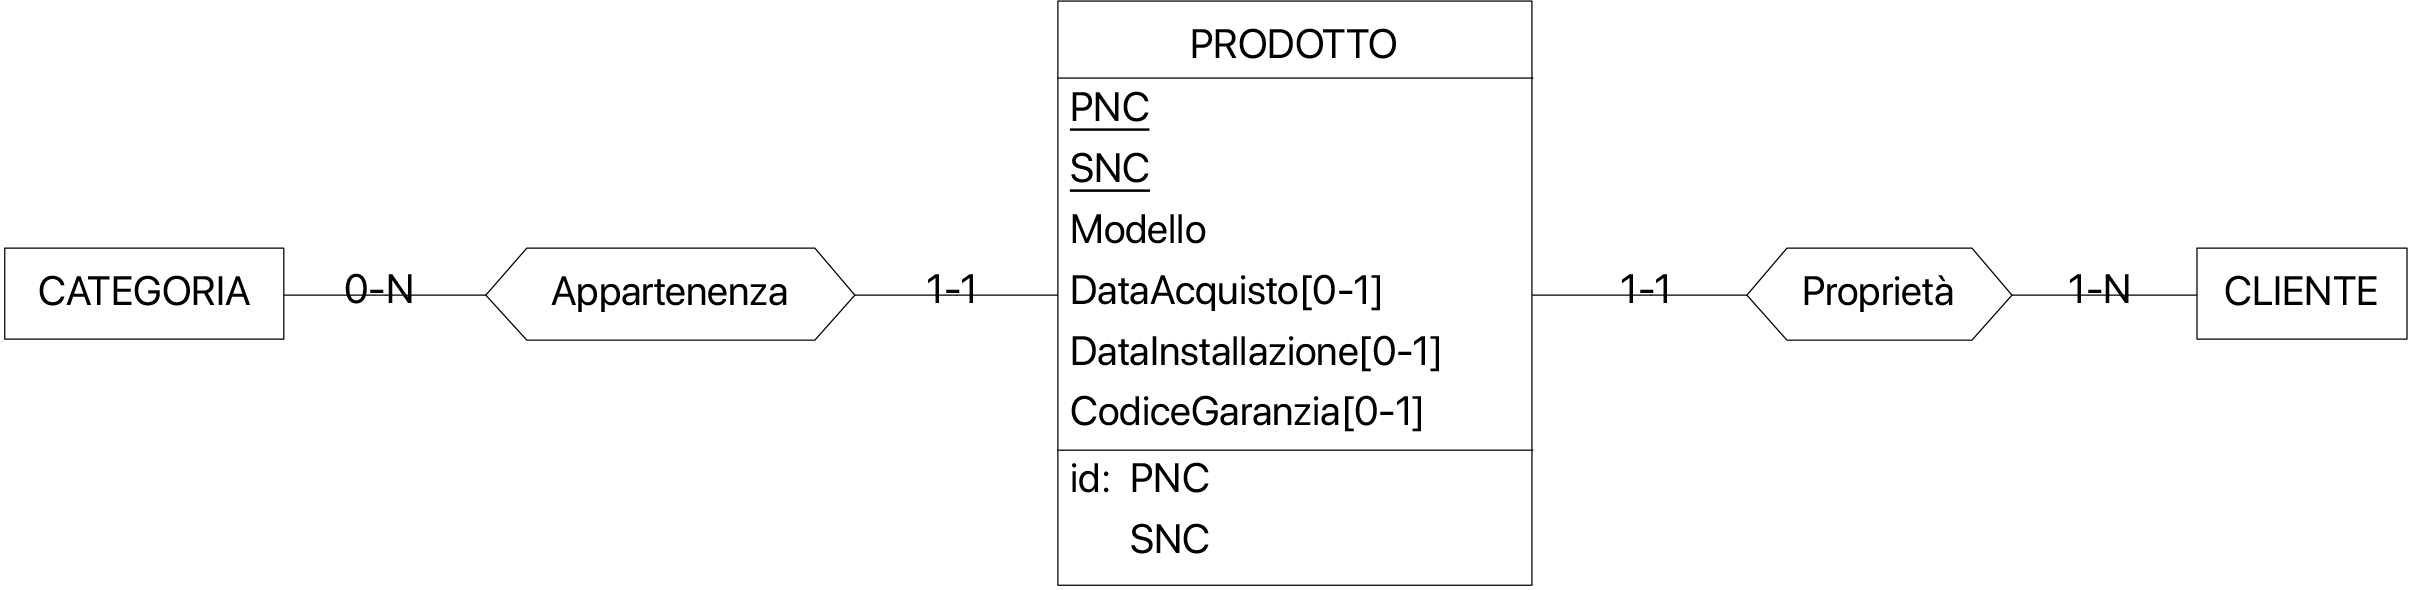
\includegraphics[width=\linewidth]{images/prodotti.png}
	\caption{Schema raffinato del concetto "prodotto" e "modello"}
\end{figure}

\section{Schema finale}

\begin{figure}[H]
	\centering
	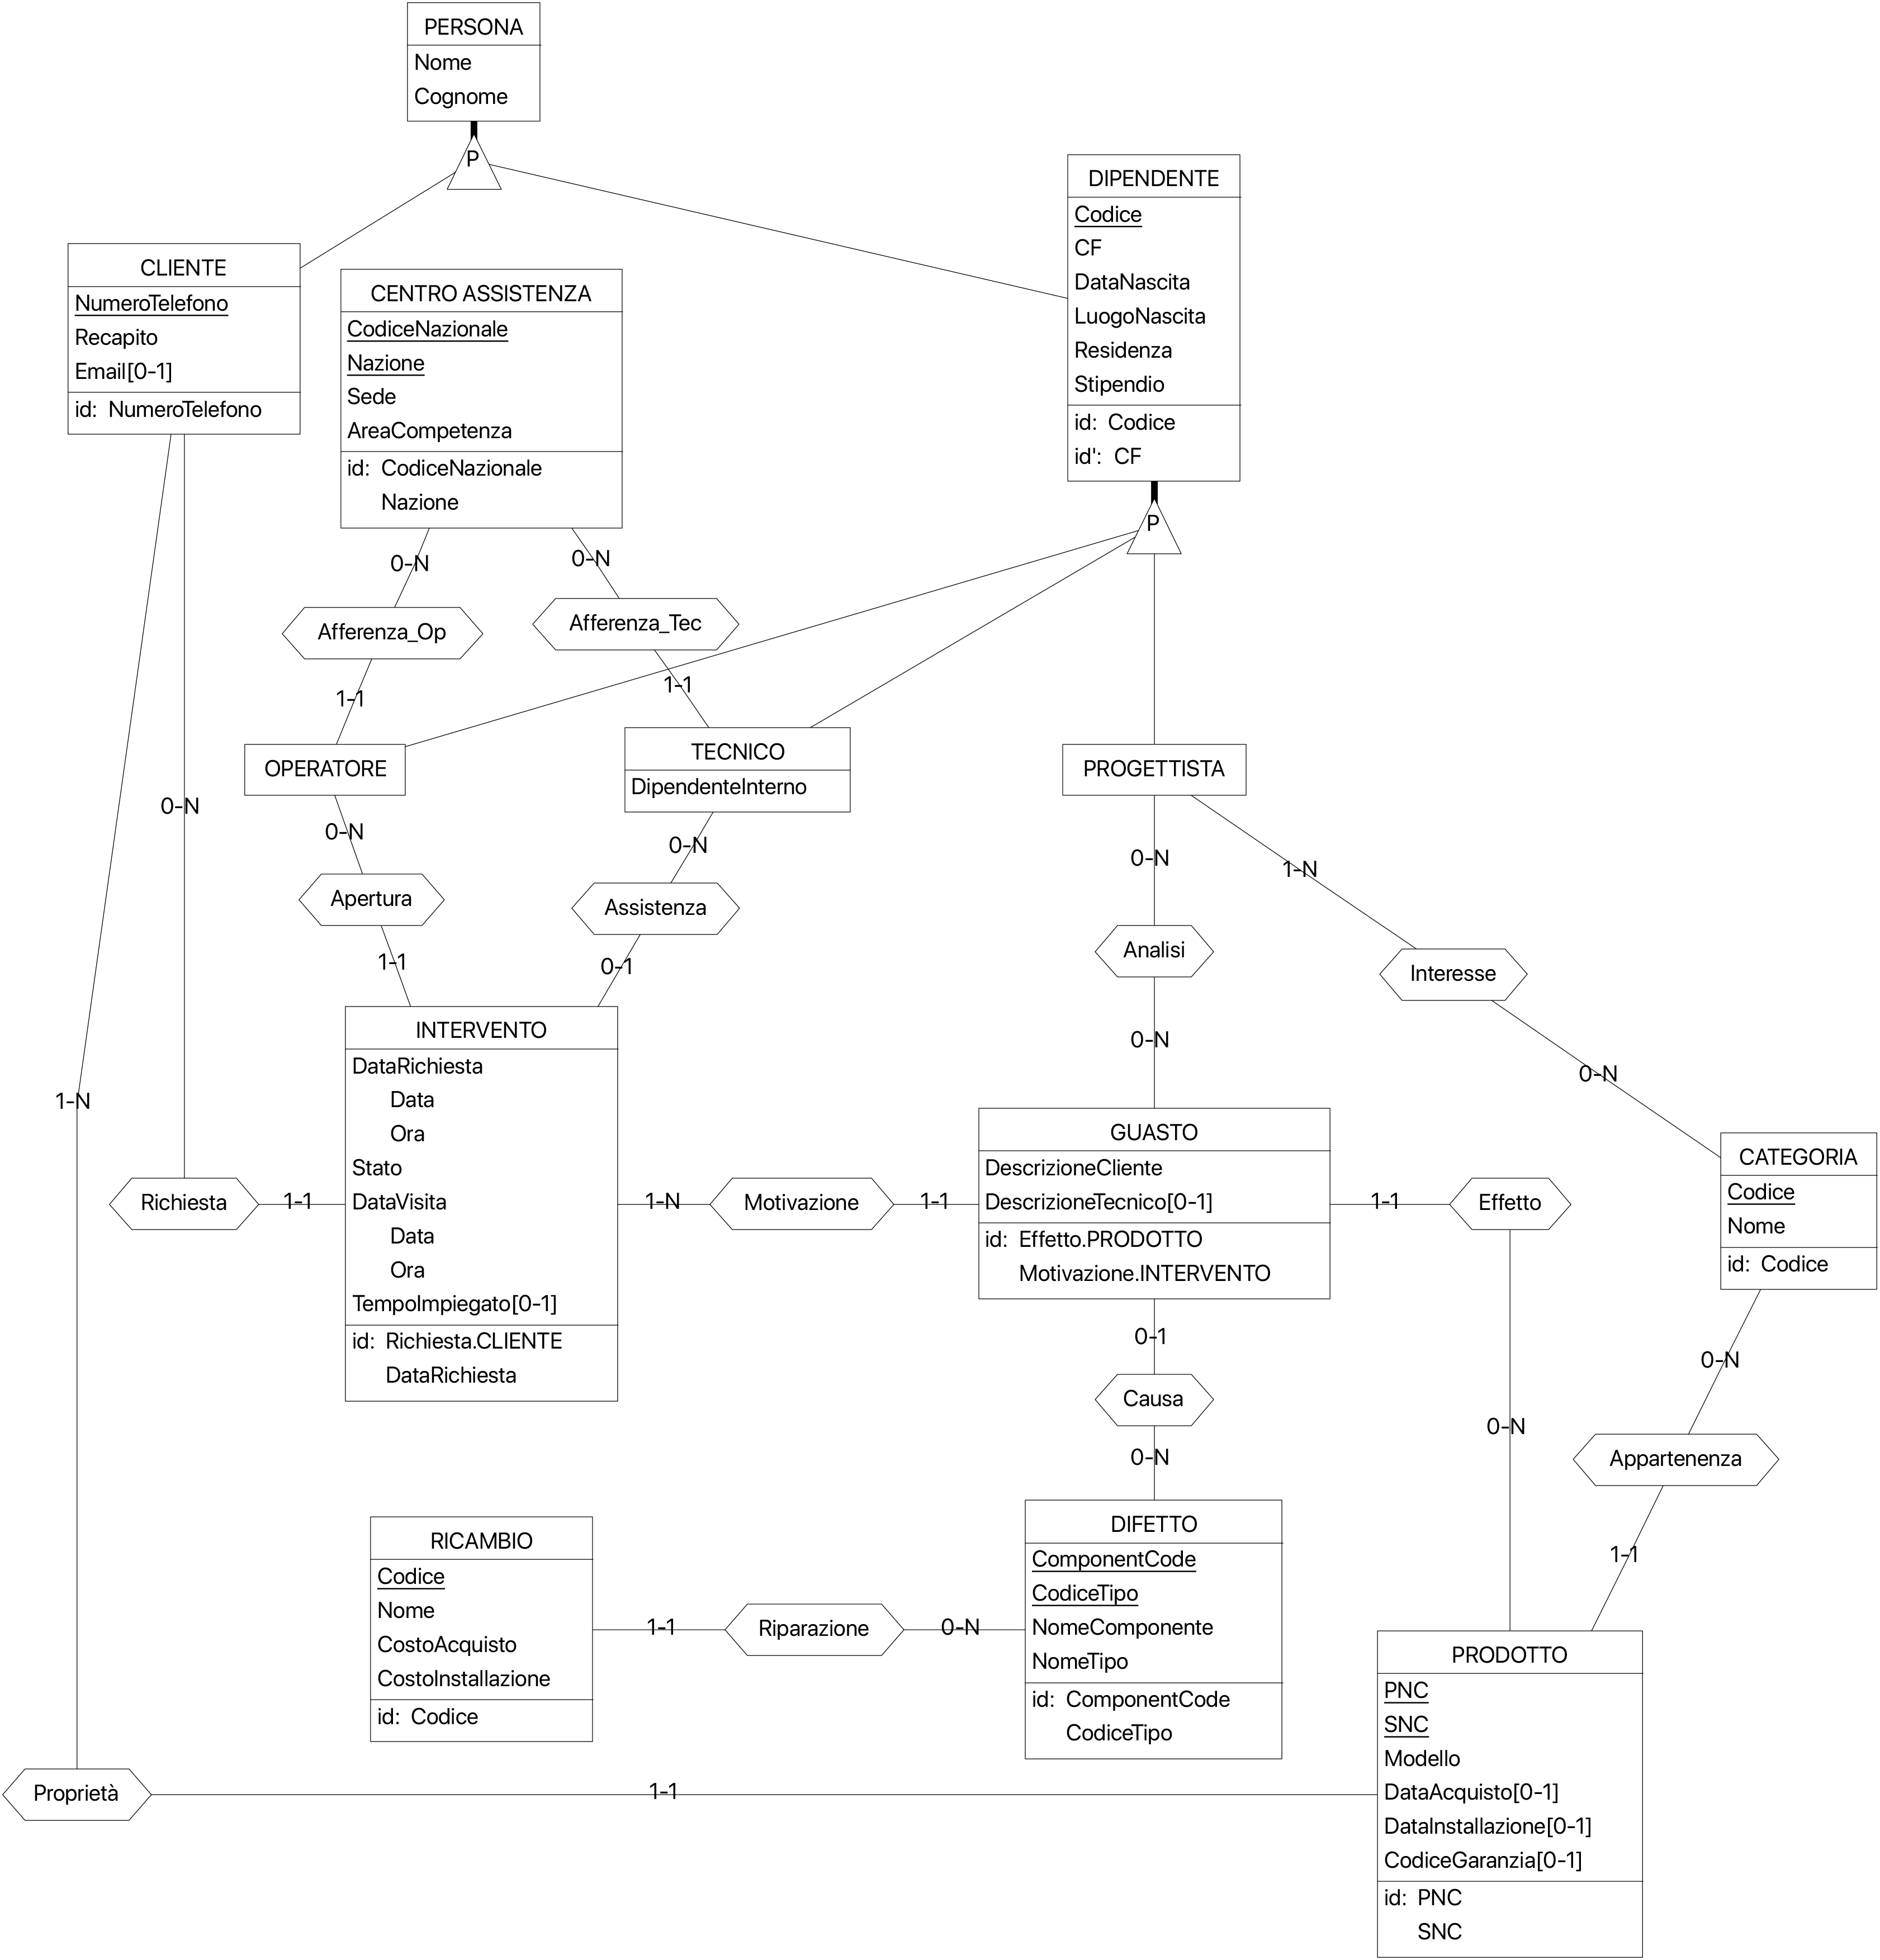
\includegraphics[width=\linewidth]{images/conceptual.png}
	\caption{Schema concettuale finale}
\end{figure}

I vincoli che questo schema non può modellare sono chiaramente quelli inerenti allo stato delle entità nel tempo, non è infatti lo schema adatto per poter
specificare chi e come dovrà modificare lo stato dell'intervento una volta creatone uno nuovo. Inoltre, non è possibile specificare nello schema che i guasti
di cui un progettista deve occuparsi sono solamente quelli che riguardano prodotti appartenenti alla sua categoria di interesse. 

\chapter{Progettazione logica}

\section{Volume dei dati}

\begin{tabularx}{\linewidth}{>{\hsize=0.375\hsize}X|X|>{\hsize=0.475\hsize}X}
	\hline
	\textbf{Nome del concetto} & \textbf{Tipo di costrutto} & \textbf{Stima del volume}\\
	\hline
	\hline
	Persona & E & \\
	\hline
	Dipendente & E & \\
	\hline
	Cliente & E & \\
	\hline
	Operatore & E & \\
	\hline
	Tecnico & E & \\
	\hline
	Progettista & E & \\
	\hline
	Centro Assistenza & E & \\
	\hline
	Afferenza_Tec & R & \\
	\hline
	Afferenza_Op & R & \\
	\hline
	Intervento & E & \\
	\hline
	Richiesta & R & \\
	\hline
	Apertura & R & \\
	\hline
	Assistenza & R & \\
	\hline
	Motivazione & R & \\
	\hline
	Guasto & E & \\
	\hline
	Analisi & R & \\
	\hline
	Difetto & E & \\
	\hline
	Causa & R & \\
	\hline
	Ricambio & E & \\
	\hline
	Riparazione & R & \\
	\hline
	Prodotto & E & \\
	\hline
	Effetto & R & \\
	\hline
	Modello & E & \\
	\hline
	Tipo & R & \\
	\hline
	Proprietà & R & \\
	\hline
	\caption{Tabella dei volumi dei dati}
\end{tabularx}

Questa tabella prende in considerazione i volumi dei dati nell'arco di ...

\section{Descrizione e frequenza delle principali operazioni}

Le principali operazioni che possono essere fatti sulla base di dati possono essere divise in tre categorie, a seconda del dipendente dell'azienda che vi accede.
In caso fosse un operatore a dover accedere, sarebbe principalmente interessato a:

\begin{itemize}
	\item[O1 -] Inserimento di un nuovo intervento
		\subitem Un operatore dovrà poter inserire un nuovo intervento 
	\item[O2 -] Cancellazione di un intervento precedentemente aperto dall'operatore stesso
		\subitem Un operatore dovrà poter cancellare un intervento aperto in precedenza da lui stesso perchè accortosi di un errore commesso nell'inserimento
		oppure perchè il cliente non desidera più ricevere alcun tipo di assistenza 
\end{itemize}

Se consideriamo invece un tecnico, le operazioni necessarie per poter svolgere la sua mansione sono:

\begin{itemize}
	\item[T1 - ] Vista di tutti gli interventi correntemente aperti non già assegnati ad un altro tecnico, ordinati per urgenza
		\subitem Prima di iniziare a lavorare, un tecnico dovrà capire quali sono gli interventi sui quali potrà dedicarsi e per poter scegliere, deve poterli avere a
		disposizione tutti quanti. In particolar modo, sarebbe più utile organizzarli per urgenza, ovvero per maggior tempo trascorso dalla data della chiamata
	\item[T2 - ] Aggiornamento di un intervento
		\subitem Una volta eseguita una riparazione, il tecnico si sarà recato a casa di un cliente e avrà perciò aggiornato le informazioni sul prodotto che il cliente
		non era riuscito a fornire. Inoltre, avrà eseguito la sua riparazione, perciò sarà necessario che aggiorni le informazioni sull'intervento di sua sola
		competenza una volta terminata la visita al cliente
\end{itemize}

Da ultimo, ci sono i progettisti che necessiteranno di stilare rapporti sotto forma di classifiche sulle principali caratteristiche dei guasti ma che competono solamente
le categorie di prodotti di loro competenza. Le principali operazioni che vorranno fare saranno:

\begin{itemize}
	\item[P1 - ] Visualizzare tutti i guasti accaduti nel mese corrente
	\subitem Ogni mese è richiesto fare un report sulla produzione degli elettrodomestici ed è perciò necessario avere a disposizione tutti i guasti che sono accaduti
	\item[P2 - ] I primi cinque modelli che hanno subito più guasti nel mese corrente
	\subitem Di tutti i guasti, quelli più importanti saranno quelli che coinvolgono i modelli più colpiti, che saranno quelli che necessiteranno un nuovo studio più urgente
	\item[P3 - ] I primi cinque \textit{PNC} che hanno subito più guasti nel mese corrente
	\subitem Ogni modello coinvolge essenzialmente più codici di prodotto più specifici e per un'analisi più di dettaglio è necessario poter avere a disposizione una classifica
	di guasti ordinata per \textit{PNC}, da cui estrarre i più "urgenti"
	\item[P4 - ] I primi cinque \textit{Component Code} che sono stati coinvolti maggiormente nei guasti di questo mese
	\subitem Alcuni componenti si guastano più di altri indipendentemente dal prodotto sul quale sono collocati. Si vuole ottenere i primi cinque maggiormente presenti questo mese
	\item[P5 - ] I primi cinque ricambi più utilizzati per riparare i guasti di questo mese
	\subitem Uno stesso ricambio può essere utilizzato in riparazioni di diversi guasti, perciò il suo costo è quello che andrà ad incidere maggiormente su quello totale dei
	ricambi acquistati per le riparazioni ed è perciò necessario stilare una classifica per ricambi utilizzati nei guasti del mese corrente.
	\item[P6 - ] I primi cinque per costo ...
\end{itemize}

\begin{tabularx}
	\hline
	\textbf{Codice operazione} & \textbf{Frequenza} & \textbf{Tipo (Interattiva / Batch)}\\
	\hline
	\hline
	O1 & & I\\
	\hline
	O2 & & I\\
	\hline
	T1 & & I\\
	\hline
	T2 & & I\\
	\hline
	P1 & & B\\
	\hline
	P2 & & B\\
	\hline
	P3 & & B\\
	\hline
	P4 & & B\\
	\hline
	P5 & & B\\
	\hline
	P6 & & B\\
	\hline
	\caption{Tabella della frequenza delle principali operazioni}
\end{tabularx}

 Nella precedente tabella vengono riassunte le frequenze di tutte le operazioni che sono state precedentemente individuate.

\section{Schemi di navigazione e tabelle degli accessi delle principali operazioni}

Per ogni operazione, verrà esplicitato a parole il modo con il quale verrà eseguita l'operazione e verrà mostrato uno schema che indichi come questi
accessi alle varie entità e relazioni si riflette sullo schema concettuale realizzato. Da questo schema, si estrarrà la tabella degli accessi che ci
permetterà di avere il costo totale di ognuna delle operazioni in termini di "\textit{I/O}".

\subsection{O1, O2 - Inserimento e cancellazione di un nuovo intervento}

L'inserimento di ogni nuovo intervento coinciderà con l'aggiunta di un nuovo intervento e, nel caso peggiore, anche di un nuovo cliente che non 

\section{Raffinamento dello schema concettuale}

\section{Analisi delle ridondanze}

\section{Traduzione di entità e associazioni in relazioni}

\section{Schema finale}

\section{Traduzione delle operazioni in SQL}

\chapter{Progettazione dell'applicazione}

\end{document}